% % % % % % % % % % % % % % 
%
%     Skript zu NUMERIK I
%           WS14/15
%    von Prof. Dr. Blank
% Universität Regensburg
%
%
%	Kap. 1: Einführung
%
% % % % % % % % % % % % % %

\marginpar{06.10.2014}
\chapter{Einführung}
\section*{Wozu?}
Oft sind Probleme mit der gleichen Struktur zu lösen,
z.B.
\begin{itemize}
\item $ax^2 + bx + c  = 0$ $\Rightarrow x_{\pm} 
  = -\frac{b}{2a} \; \pm \; \frac{1}{2a} \; \sqrt{b^2-4ac}$
\item Bestimmung des größten gemeinsamen Teilers zweier
  Zahlen \\$\leadsto$ euklidischer Algorithmus 
\end{itemize}
Hierfür ist ein allgemeiner Algorithmus erwünscht.\\

Ein weiterer Fall ist, dass ein Problem zwar analytisch gelöst werden kann, es aber
zu lange dauert bis das Ergebnis bestimmt ist,  
z.B. tauchen bei der
numerischen Simulation von Strömungen bis zu 1
Million Unbekannte auf. Damit sind Systeme mit $\approx 10^6$
Gleichungen zu lösen, wofür effiziente Algorithmen notwendig sind. \\
Näherungslösung sind bei solchen Problemen häufig ausreichend.\\

Es gibt auch Probleme, die nicht analytisch gelöst werden können, z.B.
bei Differentialgleichungen ist vielleicht Existenz- und
Eindeutigkeit gewährleistet, aber keine konstruktive Methode zur Berechnung bekannt.\\
Hierfür ist dann eine Näherungslösung gefragt.


\section*{Geschichte}
Algorithmen gibt es schon lange bevor es Rechner gab, z.B. den
euklidischen Algorithmus seit um 300 v.Chr.
\\ Die Fragestellungen
und der Blickwinkel verschieben sich jedoch in Abhängigkeit von
den zu lösenden Problemen und der 
existierenden Computer-Hardware. \\
(Strömungsprobleme modelliert mit partiellen
Differentialgleichungen,  es stehen Parallelrechner,  Vektorrechner, 
größere Speicher zur Verfügung, etc.)\\

\section*{Anwendungen}
\begin{itemize}
\item Herd, Waschmaschine, Heizungsanlage
\item Handy (über welchen Satelliten wird übertragen),
  Digitalkamera, MP3-Player
\item Navigationssysteme
\item Erstellung des Zugfahrplans
\item Robotersteuerung (bis hin zu Roboterfußball)
\item Fahrzeugindustrie
  \begin{itemize}
  \item Fahrzeugbau (Crash-Simulation,
    Strömungsmodellierung)
  \item Fahrzeugsteuerung
  \end{itemize}
\item Finanzmarkt z.B. Risikoanalyse im Wertpapierhandel
\item Klimaanalyse z.B. Vorhersage von Erdbeben, Hurrikans,
  Überflutungen
\item Medizinische Versorgung z.B. Bildverarbeitung, Prognose
  für Epedemieentwicklungen, Beschreibung des Blutkreislaufs
\item Raffinerie-Industrie
\item Kontrolle und Optimierung chemischer und biologischer
  Prozesse, z.B. Regelung von Wärmezufuhr
\item u.s.w.
\end{itemize}

\section*{Fragestellungen der Numerik}
\subsection*{Rechengeschwindigkeit \& -aufwand}
Interessant sind Rechengeschwindigkeit, Rechenaufwand 
(Anzahl der Rechenoperationen, Rechenzeit auf welchem Rechner…)
sowie Komplexität des Algorithmus.

\subsubsection{Beispiel}
Berechnung der Lösung eines Gleichungssystems 
\\ $ A x=b$ mit einer $n \times n$-Matrix $A$
\begin{enumerate}
\item Cramersche Regel\\
  $x_j = \frac{\det  (A)_j}{\det A}$ (ersetze die $j$-te
  Spalte von $A$ durch $b$)\\
  und $\det A = \sum_{\pi} \; sign (\pi) \; a_{1 m_1} \cdot \ldots \cdot a_{n
    m_n}$\\
  Benötigt etwa \textbf{n! Multiplikationen und Additionen}.
  Bei einer $20 \times 20$-Matrix $A$ (was
  heutzutage klein ist) wären dies \\
  $\approx$ 2,5
  $\cdot 10^{18}$ Operationen. Falls jede
  arithmetische Operation $10^{-6}$ Sekunden (also
  eine Mikrosekunde) benötigt, ist eine Rechenzeit
  von mehr als \textbf{eine Millionen Jahre} nötig!
\item Gaußsches Eliminationsverfahren\\
  Benötigt etwa $n^3$ Operationen, also bei einer Matrix wie oben
  ungefähr 8000 Operationen und weniger als \textbf{0,005 Sekunden}
  \cite[siehe auch][]{golubortega}.
\item Verhalten bei Störungen, Stabilität des Verfahrens
  (Eingabefehler, Rundungsfehler, Diskretisierungsfehler)\\
\end{enumerate}

\subsubsection{Beispiel}
$\frac{1}{10^{-8}} = 10^8$ Störung des Nenners $\frac{1}{2 \cdot 10^{-8}} = 5 \cdot
10^7$\\
$\leadsto$ kleine Störung im Nenner kann zu großen
Störungen im Ergebnis führen.
\\

\subsubsection{Beispiel}
$$x^2 + 314 \; x - 2 = 0$$
Falls diese Gleichung mit der \textbf{p,q-Formel} (Mitternachtsformel)
gelöst wird und immer auf 5 signifikante Stellen gerundet wird,
ergibt sich ein

{\text{\textbf{relativer Fehler}} = $\frac{|\mbox{Fehler}|}{|\mbox{Lösung}|}$}

von        $\approx 57 \; \%$.

Eine geschickte Formatierung liefert ein Ergebnis mit einem
relativen Fehler von $\approx 1,5 \cdot 10^{-5}$,
d.h. die ersten \textbf{4 Stellen sind exakt}. 
Dabei werden für $ax^2 + bx + c = 0$ folgende Ausdrücke verwendet:
\begin{align*}
  x_1 &=& \tfrac{1}{2a} \; (- b - \mbox{sign}(b) \; \sqrt{b^2 -
          4ac}\;)\\
  x_2& =  &\tfrac{2c}{- b - \mbox{sign}(b) \; \sqrt{b^2 - 4ac}} \quad .
\end{align*}
Lösung $0.0063693$, p,q-Formel $0.01$,
letzte Formel $0.0063692$

\subsection*{Genauigkeit des Verfahrens, Fehleranalyse,
  Konvergenzgeschwindigkeit, Konvergenzordnung}

\subsubsection{Beispiel}
Numerische Approximation von Ableitungen \\
Für $f \in C^3(I)$ gilt die Taylor-Entwicklung:

$f(x \pm h) = f(x) \pm h \; f'(x) + \frac{h^2}{2} \; f''(x) +
R(x)$ mit $\mid R(x) \mid \; \leq \; c   h^3$

\paragraph{Vorwärtsgenommener Differenzenquotient}
$$ (D_h^+f)(x):= \frac{f(x + h) - f(x)}{h} \; \approx f'(x), $$
$$\mid f'(x) - \frac{f(x + h) - f(x)}{h} \mid \; \leq \; c h, $$
konvergiert also mit linearer Abhängigkeit der
Schrittweite $h$  
\paragraph{Zentraler Differenzenquotient}
$$(D_h^0f) (x):= \frac{f(x + h) - f(x-h)}{2 \cdot h} \; \approx
f'(x),$$
$$\mid f'(x) - \frac{f(x + h) - f(x - h)}{2 \cdot h} \mid \;
\leq \; c h^2, $$
konvergiert mit quadratischer \textbf{Ordnung} bei
\textbf{gleichem Aufwand}!


\section*{Some desasters attributable to bad numerical computing}

{\small	(Last modified August 26, 1998 by Douglas N. Arnold,
  arnold@ima.umn.edu)}

\bigskip
{\itshape Have you been paying attention in your numerical analysis or
  scientific computation courses? 
  
  If not, it could be a costly
  mistake. 
  
  Here are some real life examples of what can happen when
  numerical algorithms are not correctly applied.}

\begin{description}
\item[The Patriot Missile failure] in Dharan, Saudi Arabia, on
  February 25, 1991 which resulted in 28 deaths, is ultimately
  attributable to poor handling of \textbf{rounding errors}. 
  
\item[The explosion of the Ariane 5 rocket] just after lift-off on its
  maiden voyage off French Guiana, on June 4, 1996, was ultimately the
  consequence of a \textbf{simple overflow}. 
  
\item[The sinking of the Sleipner] A offshore platform in Gandsfjorden near
  Stavanger, Norway, on August 23, 1991, resulted in a loss of nearly
  one billion dollars. It was found to be the result of
  \textbf{inaccurate finite element analysis.} 
\end{description}

\section*{Weitere praxisrelevante Fragestellungen}
\begin{itemize}
\item Nutze black box solver oder entwickle Lösungsmethode,
  welche auf das spezielle Problem angepaßt ist.
\item Wie teuer ist die Implementierung? \\(= wieviel Arbeitszeit)
\item Ist der implementierte Algorithmus vielseitig einsetzbar?\\
  (welche Problemklassen deckt er ab, welche Rechnerstruktur ist
  vorausgesetzt)
\end{itemize}

\section*{\enquote{Gute} Programme}
\begin{itemize}
\item zuverläßig (fehlerfrei)
\item robust (z.B. behandeln Ausnahmesituationen und filtern
  ungeeignete Daten heraus)
\item portierbar auf andere Rechenanlagen
\item wartungsfreundlich (leicht zu ändern oder zu erweitern)
\item gut dokumentiert
\item ausgiebig getestet \\   
  {\small \it soll in den Übungen trainiert werden}
\end{itemize}

\paragraph{Eine Faustregel der numerischen Mathematik}~\\
Zu jedem noch so eleganten numerischen Verfahren gibt es ein Gegenbeispiel,
für welches die Methode völlig versagt. \\
{\tiny(Teubner Taschenbuch)}

\section*{Welche Probleme werden hier behandelt?}
\begin{enumerate}
\item \textbf{Lineare Gleichungssysteme} $Ax=b$ 
  \begin{itemize}
  \item \enquote{kleine} bis \enquote{mittelgroße} Matrizen\\
    $\rightarrow$ \textbf{direkte Methoden:} nach endlich vielen
    Schritten ist die \textbf{exakte Lösung} bis auf
    Rundungsfehler berechnet (z.B. Gauß-Elimination)
  \item strukturierte Matrizen \\
    Symmetrie oder sogar Bandstruktur:
    \begin{image}{Bandmatrix}
      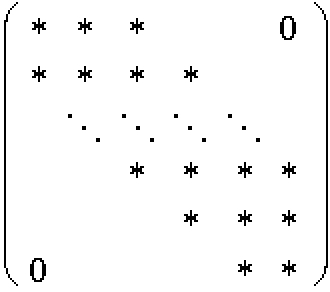
\includegraphics[width=5cm]{images/band.jpg}  
    \end{image}
    
    
  \item große Matrizen (mit zusätzlichen Eigenschaften)\\
    $\rightarrow$ \textbf{iterative Methoden:} kenne Startwert
    $x_0$, berechne neue Approximation $x_i$ unter
    Ausnutzung der vorherigen bis die
    \textbf{Näherungslösung} $x_i$ \enquote{gut genug ist}.
  \end{itemize}
  
\item \textbf{Lineare Ausgleichsprobleme}\\
  Beispiel:\\
  Wir messen den Zusammenhang zwischen Spannung U und
  Stromstärke I
\begin{image}{Einfacher Stromkreis}
  \parbox[c]{3cm}{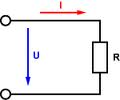
\includegraphics[width=2cm]{images/ohmsche.jpeg} }
\end{image}
\begin{image}{Linearausgleich von Messwerten}
  \parbox[c]{6cm}{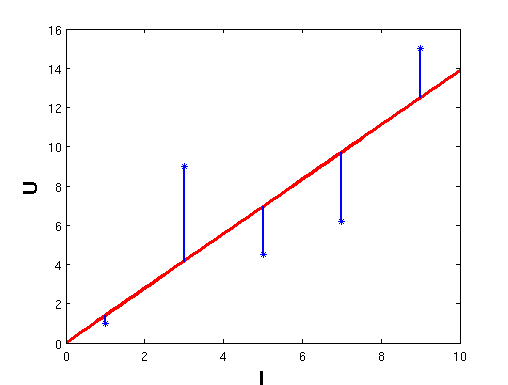
\includegraphics[width=5cm]{images/linausgl2.png}}
\end{image}
  Ohmsches Gesetz: $U = R \cdot I$\\
  Gesucht ist der Widerstand R. \\
  ($U_i, I_i$) seien die Messdaten mit möglichen Messfehlern.\\
  Finde nun $R$, sodass 
  $\; f(R)\, =\,  \min\limits_r \; \sum\limits_i \; (U_i - r \; I_i)^2$
  
\item \textbf{Lösung nichtlinearer Gleichungen},
  z.B.
  \begin{itemize}
  \item Berechnung von Nullstellen $g(x) = 0$
  \item Berechnung von Fixpunkten $f(x) = x$
  \end{itemize}  
\item \textbf{Eigenwertwertberechnung}
  $\quad Ax= \lambda x, \qquad \; \lambda \in \mathbb{C}$
  
  
\item \textbf{Interpolation}\\
  Setze Meßdaten zu einer kontinuierlichen Funktion fort, \\
  aber wie \enquote{glatt}?\\
  z.B. stückweise konstant, stückweise linear, oder 
  falls sie
  eine Schwingung repräsentieren, berechne die zugehörige
  Fourierreihe  
  
\item \textbf{Berechnung von Integralen} (Quadraturformeln) \\ 
  Approximation von $\int_a^b \; f(x) \; dx$
\end{enumerate}~\\

Bei allem spielt die \textbf{Fehleranalyse} eine große Rolle und
ihre Grundbegriffe werden in einem extra Abschnitt behandelt.

%%% Local Variables:
%%% mode: latex
%%% TeX-master: "../numerik_script"
%%% End:
